\section{実験装置}
以下に実験に使用した装置およびスキャンした収穫物を示す.
3Dスキャナは非接触式でハンディタイプのArtec Leoを使用した.
スキャンした収穫物は, \figref{Fig:plant}に示すようなハウス内で栽培されているピーマン株である.
また, Blenderを用いてピーマンの3Dモデルから特性を計測した.

\vspace{5mm}
\begin{figure}[H]
     \centering
     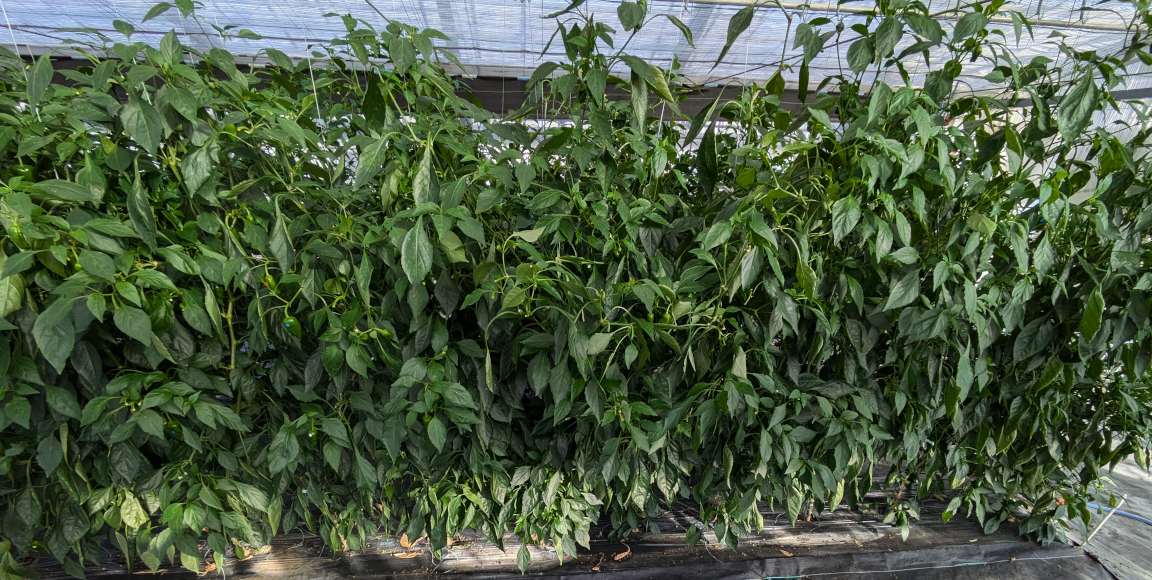
\includegraphics[width=110mm]{images/png/plant.png}
     \caption{Scanned plants}
     \label{Fig:plant}
   \end{figure}